% CVPR 2022 Paper Template
% based on the CVPR template provided by Ming-Ming Cheng (https://github.com/MCG-NKU/CVPR_Template)
% modified and extended by Stefan Roth (stefan.roth@NOSPAMtu-darmstadt.de)

\documentclass[10pt,twocolumn,letterpaper]{article}

%%%%%%%%% PAPER TYPE  - PLEASE UPDATE FOR FINAL VERSION
%\usepackage[review]{cvpr}      % To produce the REVIEW version
%\usepackage{cvpr}              % To produce the CAMERA-READY version
\usepackage[pagenumbers]{cvpr} % To force page numbers, e.g. for an arXiv version

% Include other packages here, before hyperref.
\usepackage{graphicx}
\usepackage{amsmath}
\usepackage{amssymb}
\usepackage{booktabs}
\usepackage{multirow}


% It is strongly recommended to use hyperref, especially for the review version.
% hyperref with option pagebackref eases the reviewers' job.
% Please disable hyperref *only* if you encounter grave issues, e.g. with the
% file validation for the camera-ready version.
%
% If you comment hyperref and then uncomment it, you should delete
% ReviewTempalte.aux before re-running LaTeX.
% (Or just hit 'q' on the first LaTeX run, let it finish, and you
%  should be clear).
\usepackage[pagebackref,breaklinks,colorlinks]{hyperref}


% Support for easy cross-referencing
\usepackage[capitalize]{cleveref}
\crefname{section}{Sec.}{Secs.}
\Crefname{section}{Section}{Sections}
\Crefname{table}{Table}{Tables}
\crefname{table}{Tab.}{Tabs.}


%%%%%%%%% PAPER ID  - PLEASE UPDATE
\def\cvprPaperID{*****} % *** Enter the CVPR Paper ID here
\def\confName{CVPR}
\def\confYear{2022}


\begin{document}

%%%%%%%%% TITLE - PLEASE UPDATE
\title{Turning Noise into Treasure:\\ A Complementary Label Learning Approach for Noisy Labels}

% \author{First Author\\
% Institution1\\
% Institution1 address\\
% {\tt\small firstauthor@i1.org}
% % For a paper whose authors are all at the same institution,
% % omit the following lines up until the closing ``}''.
% % Additional authors and addresses can be added with ``\and'',
% % just like the second author.
% % To save space, use either the email address or home page, not both
% \and
% Second Author\\
% Institution2\\
% First line of institution2 address\\
% {\tt\small secondauthor@i2.org}
% }
\author{Meng Pan\\ School of Computer Science and Engineering, Sun Yat-sen University, China\\{\tt\small \{panm9\}@mail2.sysu.edu.cn}}

\maketitle

%%%%%%%%% ABSTRACT
\begin{abstract}
\end{abstract}

\section{Introduction}
Monocular Depth Estimation is a crucial 3D scene perception algorithm. 
Trapped by the lack of sufficient geometric constraints, 
MDE is still an ill-posed problem. With the rapid development of 
Deep Neural Networks(DNNs), MDE has emerged many excellent works 
in recent years. However, according to Szegedy's research, DNNs are 
prone to be attacked by adversarial examples: when a imperceptibly 
small perturbation is added to an input image, the classifier 
based on DNNs will classify the image into a wrong category with high probability. 
This property has been verified not only on classification tasks, 
but also on logical regression tasks, such as semantic segmentation and 
object recognition. MDE also failed to get rid of this dilemma.

As a kind of 3D scene perception algorithm, MDE needs to be 
robust and reliable, so that when an attack occurs in automatic 
driving, the vehicle can still accurately perceive the depth 
of the scene. Otherwise, the damage is much more serious than 
the percentage loss in accuracy. On MDE, this problem was 
first confirmed and researched by Wong. They conducted 
comprehensive and rigorous experiments to explore the impact 
of pixel attacks on MDE. Including attacking the whole 
depth map of a scene, attacking the depth map of one 
single object in the scene, and even making a specific 
object vanished completely on the depth map by 
adding perturbations. This research is pioneering and 
enlightening for attacking MDE.

However, the study of Wong can hardly apply to physical 
world, it didn't take physical attack into account. 
The perturbations used in experiments are elaborately designed, 
which are very hard to realize in the physical world. 
While attacking a scene by patch is an appropriate solution: 
sticking a patch into the scene to be attacked is much more 
reasonable and implementable.
Some researches exploit patches to attack DNNs, but most of them 
didn't pay much attention on inconspicuousness. 
Abrupt and unreal patch in scenes will reveal the attack 
intention.
Indeed, some works noticed this problem and utilize GAN to make patches
more naturalistic. 
This will increase time and space complexity obviously.
In this study, we take physical realizability and 
inconspicuousness into accout, design an algorithm to attack MDE.

Specifically, we design a learnable matrix, 
which can generate reasonable patches according to depth map 
automatically. The generation processes are driven by three 
learnable coefficients and don't need any extra generation networks.

\section{Related Work}
In this work, patch attacks of MDE model are concentrated on, 
so a brief review of MDE and patch attacks will be 
introduced in this section.

\subsection{Monocular Depth Estimation}
\subsubsection{Supervised}
DNNs learn through the supervision of ground truth labels 
annotated artificially. Since the mapping from a single image 
to a depth map is very complicated, this supervised learning 
manner is very suitable for MDE tasks. The initial work adopts 
this \textbf{intuitive endoder-decoder} concept. 
Eigen et al designed two hierarchical neural networks to predict 
the depth map in coarse and fine respectively.
A network was proposed subsequently by them, in which three 
different tasks, depth estimation, segmentation and 
normals prediction was integrated into one model.
Lee coined novel local planar guidance layers and locate 
them at different scale decoding phases. 
As a result of this, final fine depth maps are densely 
restored from small to big.
Current MDE networks are bulky and inefficient, which can not
be equipped on embedding systems. Wofk et al. proposed Fashdepth,
a light, fast MDE network.
Some researches address this problem by formulizing it as 
a \textbf{classification} problem. 
Discrete depth labels are prepared by separating 
continuous depth value, which are then used to supervise 
the training process.
While using \textbf{relative depth information} to predict depth 
indirectly is also a effective solution.
Lee proposed a method to predict depth from relative depth. 
They first estimate relative depth by utilizing rank-1 property, 
then the final depth maps are reconstructed through these relative 
depth maps.

\subsubsection{Unsupervised}
Although there exist some datasets with ground truth depth 
annotation, dense and accurate depth maps are labor-consuming and rare. 
In that case, unsupervised methods dominate recently.
Godard et al. exploit the left-right consistency of binocular image pairs
to tackle this issue: 
with a decently predicted disparity, 
the two images sampled from a binocular camera can synthesize each other. 
A consecutive vedio sequence can provide a constrain for MDE.
Given a middle frame and its former, later frame sampled from a video, 
DNNs can estimate the camera pose and the depth, with which we can 
restore the other two frames. Based on this constrain, camera pose 
and depth can be learned jointly.
However, there is a flaw in both video and binocular solutions.
On the one hand, binocular image pairs methods struggle in occlusion 
and texture-copy problems, yet, on the other hand, as an alternative method, 
predicting depth from a video performs unsatisfactorily 
when it comes to relatively stationary objects.
To address this, Godard et al. proposed a multi-scale reconstruction
loss and a automasking approach to ignore relatively stationary objects.
\subsection{Patch Attack}
Adding perturbations to images has a limit: 
the imperceptive noise can not be captured by camera.
Recently, researchers turn to generating adversarial examples with
patches. It can be captured by camera and it can implement to physical
world. The only question is, how to make it concealed.

Mahmood et al. attacked FRS using real printed glass frames, 
with which the FRS can not recognize the person or recognize him
as someone else in the system. The pattern of these frames are
generated optimizied by an objective function.

\section{Approach}
In this section, we first introduce some preliminaries about our noisy label learning. Subsequently, we give a brief introduction to our baseline method DivideMix\cite{li2020dividemix}. Finally, we illustrate our proposed complementary label learning approach.
\subsection{Preliminaries}
\paragraph{Problem formulation.}We define the task of K-category classification with noisy labels. Formally, we denote the labeled dataset $\mathbb{D}=\left\{\left(x_{i}, y_{i}\right) \mid 1 \leq i \leq N\right\}$, in which $ x_{i} \in \mathcal{X}$ is the i-th training sample and $ y_{i} \in \mathcal{Y}$ is the corresponding label over $ K $ classes with noise. Normally, a supervised classification learns a function $f: \mathcal{X} \rightarrow \mathcal{Y}$ that maps the input space to label space. The common objective loss function that used to define the empirical risk is the Cross-Entropy(CE) loss function:
\begin{equation}\label{ce}
\mathcal{L}_{C E}(f,y)=-\frac{1}{N} \sum_{i=1}^{N} \sum_{k=1}^{K} y_{i}^{k} \log \left(p_{i}^{k}\right)
\end{equation}
in which $ p_{i}^{k} $ is the predicted probability of sample $ x_{i} $ for class $ k $. The objective of training classifier is to find the optimal parameters $ \theta $ that minimize the objective loss function. And our target is to train a classifier robust to the noisy label in training set.
\paragraph{Sample-selection-based methods.} A common idea of dealing with noisy labels is sample-selection-based method, which aims to determine which samples may be noisy. Such methods need to find a reliable selector to distinguish the clean samples and noisy samples, and then either discard noisy samples directly or reassign labels for them. The challenging issue is to design a reliable criteria to select clean samples. Previous works have shown that deep neural networks(DNNs) tend to learn simple pattern first before fitting label noise\cite{arpit2017closer}. Therefore, lots of methods treat samples with large loss as noisy samples and construct new pseudo labels for them like semi-supervised learning.
\subsection{Baseline: DivideMix}
Our baseline method is DivideMix\cite{li2020dividemix} which is a typical sample selection based method. DivideMix uses a mixture model to model the per-sample loss distribution so that it can divide the training data into a labeled set with clean samples and an unlabeled set with noisy samples dynamically. Besides, to avoid confirmation bias of self-training, that is, the model would accumulate its errors, DivideMix train two networks at the same time to filter errors through epoch-level implicit teaching and batch-level explicit teaching. Specifically, at each epoch, DivideMix perform co-divide, in which one network divides the noisy training dataset into clean labeled set and noisy unlabeled set, which are then used by the other network. At each mini-batch, utilizes both labeled and unlabeled samples are utilized by one network to perform semi-supervised learning guided by the other network. 
\subsection{Our negative losses}
DivideMix has achieved remarkable performance on many large-scale datasets with both symmetric and asymmetric label noise. However, it does not make good use of the labels of noisy samples, but directly assign pseudo labels for them. In order to further utilize the label of noisy samples, we propose to adopt complementary label learning\cite{ishida2017learning} approach that utilize noisy labels as complementary labels to serve as an additional robust supervised signal after sample selection. Our approach is based on two basic assumptions:
\begin{itemize}
\item[1)] Designing a reliable sample detector is feasible because DNNs tend to learn common patterns first and then memorize the noisy data\cite{arpit2017closer}.
\item[2)] Given a reliable sample selector, we are more sure of what an image isn't than what it is.
\end{itemize}
Based on the two assumptions, we apply the complementary label learning after sample selection. For noisy sample, the original label now serves as the complementary label and the output probability of it is suppressed explicitly. Specially, given the label $ \tilde{y}_{i} $ of a noisy sample , we can define $ q_{i}^{k} = 1 - p_{i}^{k} $, which means the probability that the sample does not belong to class $ k $. Then we treat the label $ \tilde{y}_{i} $ of a noisy sample as the label that it does not belong to this class and calculate the loss with $q_{i}^{k}$.
\paragraph{Negative-CE(Neg-CE).} We can use Cross-Entropy loss function to measure the difference between predicted $ q_{i}^{K}$ and label $ \tilde{y}_{i} $ of a noisy sample:
\begin{equation}\label{negce}
\mathcal{L}_{Neg-CE}(f,\tilde{y})=-\frac{1}{N} \sum_{i=1}^{N} \sum_{k=1}^{K} \tilde{y}_{i}^{k} \log \left(q_{i}^{k}\right)
\end{equation}
\paragraph{Negative-MSE(Neg-MSE).} We can also use mean square error(MSE) instead of Cross-Entropy loss, the Neg-MSE loss function for noisy labels can be defined as:
\begin{equation}\label{negmse}
\mathcal{L}_{Neg-MSE}(f,\tilde{y})=-\frac{1}{NK} \sum_{i=1}^{N} \sum_{k=1}^{K} (q_{i}^{k}-\tilde{y}_{i}^{k})^{2}
\end{equation}
Our proposed Neg-CE or Neg-MSE loss function can be combined with arbitrary existing sample-selection methods by simply adding the Neg-CE/MSE loss term. 

\section{Experiments}
In this section, we would like to answer the following questions: (1) how does the loss function compare to the baseline? (2) Is the loss function robust and efficient enough for different noisy label ratios and different noisy label types?
To answer these question, we evaluate our method on CIFAR-10 datasets~\cite{krizhevsky2009learning}. We apply our loss function to DivideMix~\cite{li2020dividemix} and compare our model to the naive model in different sets.

\subsection{Datasets and Label Noise Types}    
\paragraph{CIFAR-10~\cite{krizhevsky2009learning}.}To demonstrate the capability of the loss function, we conduct experiments on CIFAR-10, consisting of 32$\times$32 color images arranged in 10 classes. The datasets contains 50,000 training and 10,000 test images.
\paragraph{Label Noise Types.}For CIFAR-10, we use two types of label noise to mix up: symmetric and asymmetric. \textbf{Symmetric}: The label has equal probability to flip to another class. Following~\cite{he2016deep}and~\cite{tanaka2018joint}, we generate noisy label by convert the labels of a give training data to one of the other classes using the set proportion(the ground truth labels are randomly scrambled). \textbf{Asymmetric}: The label was only changed to a specific class. For example, we choose the train sample randomly with a set probability and change the label to its similar class ({\eg} \textbf{BIRD} $\rightarrow$ \textbf{AIRPLANE}), \textbf{CAT} $\rightarrow$ \textbf{DOG}, \textbf{HORSE} $\rightarrow$ \textbf{DEER}, same to the setting in~\cite{yao2019safeguarded}.

For comparing the methods, we mix up the datasets under asymmetric noise rate of $\eta_{a s y m m}\in\{0.4\}$ and the symmetric noise rates of $\eta_{s y m m}\in\{0.2,0.5,0.8,0.9\}$.
\subsection{Implementation Details}
\paragraph{Hyperparameters.}For implementation on CIFAR-10, we set the batch size to 64 and use an 18-layer Pre-Train Resnet~\cite{he2016identity}. Training it use stochastic gradient descent (SGD), momentum of 0.9, weight decay of $5e^{-4}$, and a batch size of 64. Besides, we train the two networks for 300 epochs. The initial learning rate is set to 0.02, and was reduced by a factor 10 after 150 epochs. For Warm up the network, the period is 10 epochs for CIFAR-10. 
\paragraph{Data Argumentation.}In order to enhance the diversity and richness of the data and enable the network to learn more robust features, we performed normalize, random horizontal, and random crops for CIFAR-10.

The Hyperparameters and Data Augmentation are the same with baseline~\cite{li2020dividemix}.

\begin{table*}[!t]
\makeatletter
\centering
\resizebox{4in}{!}{
\begin{tabular}{cc|cccc|cl}
\toprule
\multicolumn{2}{c|}{\multirow{2}{*}{Method/Noise}}     & \multicolumn{4}{c|}{symmetric} & \multicolumn{2}{c}{asymmetric} \\ \cline{3-8} 
\multicolumn{2}{c|}{}                                  & 0.2    & 0.5   & 0.8   & 0.9   & \multicolumn{2}{c}{0.5}        \\ \hline
\multicolumn{1}{c|}{\multirow{2}{*}{DivideMix\cite{li2020dividemix}}} & Avg  & \textbf{95.7}   & \textbf{94.4}  & 92.9  & 75.4  & \multicolumn{2}{c}{92.1}       \\
\multicolumn{1}{c|}{}                           & Best & \textbf{96.1}   & \textbf{94.6}  & 93.2  & 76.0  & \multicolumn{2}{c}{\textbf{93.4}}       \\ \hline
\multicolumn{1}{c|}{\multirow{2}{*}{+Neg-MSE}}   & Avg  & 95.6   & 94.3  & \textbf{93.2}  & \textbf{77.8}  & \multicolumn{2}{c}{\textbf{92.9}}       \\
\multicolumn{1}{c|}{}                           & Best & 95.8   & \textbf{94.6}  & \textbf{93.5}  & \textbf{79.2}  & \multicolumn{2}{c}{\textbf{93.4}}       \\ \hline
\multicolumn{1}{c|}{\multirow{2}{*}{+Neg-CE}}    & Avg  & 95.2   & 93.5  & 92.4  & 77.0  & \multicolumn{2}{c}{92.1}       \\
\multicolumn{1}{c|}{}                           & Best & 95.5   & 94.1  & 92.6  & 78.5  & \multicolumn{2}{c}{92.6}             \\
\bottomrule
\end{tabular}
}
\caption{Comparison with baseline method on CIFAR-10 mixed with various types and ratios of noise.}
\label{table:exp}
\end{table*}


\subsection{Quantitative Results}
Table \ref{table:exp} shows the results of our method and baseline method in various noise types and ratios on CIFAR-10. The result shows baseline method has a high accuracy in the low noisy environment, but the performance decreases drastically as the noise ratio increases. Our method (\textbf{Neg-MSE}) obtained an improvement compared to the baseline method when the noise ratio is high. But the performance is not good enough when the set comes to low noise ratio (\eg 0.2,0.5). In addition, compared to the cross entropy, MSE Loss is much more robust to various label noise ratio.

\begin{figure*}[!htbp]
	\centering
	\subfloat[CIFAR-10-Sym-Noise20$\%$]{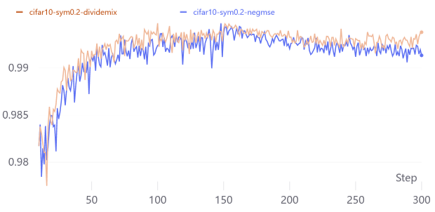
\includegraphics[width=0.4\linewidth]{./imgs/acc1.png}\label{fig:acc-a}}\quad
	\subfloat[CIFAR-10-Sym-Noise50$\%$]{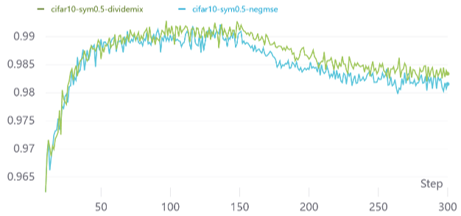
\includegraphics[width=0.4\linewidth]{./imgs/acc2.png}\label{fig:acc-b}}\\
	\subfloat[CIFAR-10-Sym-Noise80$\%$]{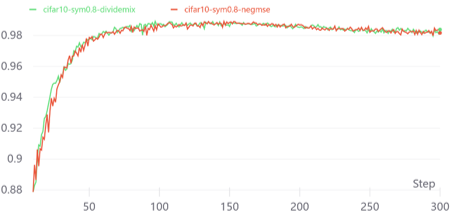
\includegraphics[width=0.4\linewidth]{./imgs/acc3.png}\label{fig:acc-c}}\quad
	\subfloat[CIFAR-10-Sym-Noise90$\%$]{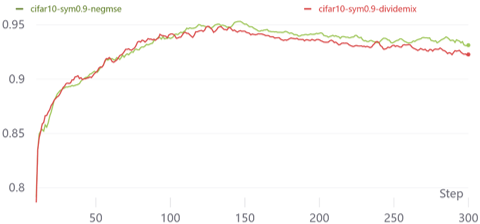
\includegraphics[width=0.4\linewidth]{./imgs/acc4.png}\label{fig:acc-d}}\\
	\caption{Accuracy graph of Negmse(our) and DivideMix with CIFAR-10 mixed with 20$\%$, 50$\%$, 80$\%$, and 90$\%$ symmetric noise.}
	\label{fig:Acc}
\end{figure*}

\subsection{Further Analysis}
\paragraph{Results on CIFAR-10.}Fig.\ref{fig:Acc} shows the accuracy graph of Negmse (our) and DivideMix with CIFAR-10 mixed with 20$\%$, 50$\%$, 80$\%$, and 90$\%$ symmetric noise. As can be seen in Fig.\ref{fig:Acc}, training with negative Mse can improve the AUC of clean/noiey selection in high noise radio setting (bottom), but reduce it in low noise radio setting (top). That's to say, the negative Mse tends to let the network makes more false positive predictions than the baseline under low noise radio.

we have two Hypothesis to explain the performance of our loss function on CIFAR-10. Firstly, false positive samples dominate the gradient of negative MSE loss. Assuming that, the similarity between distribution of prediction and label of false positive data is larger than that of true noisy data. So, the negative MSE would produce greater gradients on these false positive samples then the true label samples. But the optimization direction for these samples is most likely to be wrong. When the noisy ratio comes to low, the nework in a much stronger wrong direction will have  a lower accuracy in true positive data then before. Secondly, training in low noise ratio is more sensitive to false positive samples compared to high loss ratio,since the number of true noisy sample is less, which will enhance the influence of false positive samples.

\section{Conclusion}
In this paper, we apply the complementary label learning to further utilize the noisy labels to strengthen the training of existing sample-selection methods, instead of discarding them. From the empirical results, we observe that it works well on high noise ratio, but gets trouble on low noise rate. We think the underlying reason is related to the influence of FP samples. In a word, the results on high noise ratio show the effectiveness of our approach, but the influence of FP samples needs to be alleviated, which is the focus of our future work.

We then speculate that the reason for poor performance under low noise rate is the influence of false positive (FP) samples(\ie,clean samples which are misjudged as noise). 


%%%%%%%%% REFERENCES
{\small
\bibliographystyle{ieee_fullname}
\bibliography{egbib}
}

\end{document}
